\begin{center}
\end{center}



\tikzset{every picture/.style={line width=0.75pt}} %set default line width to 0.75pt        

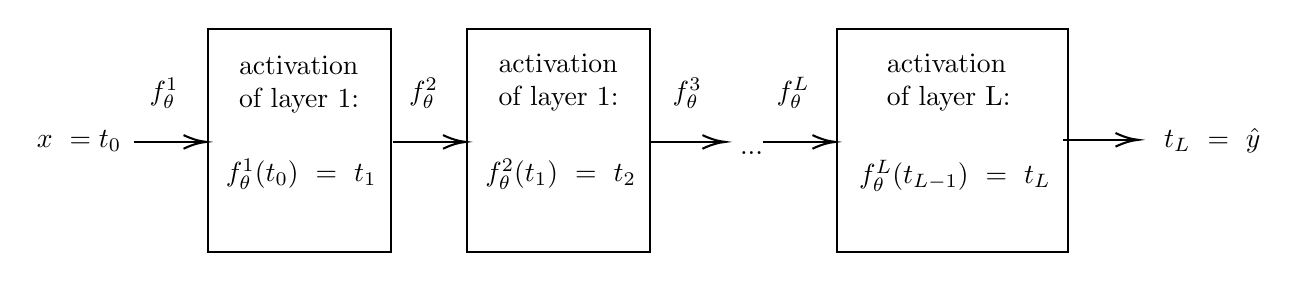
\begin{tikzpicture}[x=0.75pt,y=0.75pt,yscale=-1,xscale=1]
%uncomment if require: \path (0,244.52349853515625); %set diagram left start at 0, and has height of 244.52349853515625

%Shape: Rectangle [id:dp11557839760136379] 
\draw   (86,115) -- (174.28,115) -- (174.28,222.54) -- (86,222.54) -- cycle ;
%Straight Lines [id:da1142035093360374] 
\draw    (50.28,169.54) -- (83.28,169.54) ;
\draw [shift={(85.28,169.54)}, rotate = 180] [color={rgb, 255:red, 0; green, 0; blue, 0 }  ][line width=0.75]    (10.93,-3.29) .. controls (6.95,-1.4) and (3.31,-0.3) .. (0,0) .. controls (3.31,0.3) and (6.95,1.4) .. (10.93,3.29)   ;

%Straight Lines [id:da3402708303870947] 
\draw    (299.28,169.54) -- (333.28,169.54) ;
\draw [shift={(335.28,169.54)}, rotate = 180] [color={rgb, 255:red, 0; green, 0; blue, 0 }  ][line width=0.75]    (10.93,-3.29) .. controls (6.95,-1.4) and (3.31,-0.3) .. (0,0) .. controls (3.31,0.3) and (6.95,1.4) .. (10.93,3.29)   ;

%Straight Lines [id:da9984222042248518] 
\draw    (498.28,168.54) -- (532.28,168.54) ;
\draw [shift={(534.28,168.54)}, rotate = 180] [color={rgb, 255:red, 0; green, 0; blue, 0 }  ][line width=0.75]    (10.93,-3.29) .. controls (6.95,-1.4) and (3.31,-0.3) .. (0,0) .. controls (3.31,0.3) and (6.95,1.4) .. (10.93,3.29)   ;

%Shape: Rectangle [id:dp7529094555455995] 
\draw   (211,115) -- (299.28,115) -- (299.28,222.54) -- (211,222.54) -- cycle ;
%Straight Lines [id:da3983438928921348] 
\draw    (175.28,169.54) -- (208.28,169.54) ;
\draw [shift={(210.28,169.54)}, rotate = 180] [color={rgb, 255:red, 0; green, 0; blue, 0 }  ][line width=0.75]    (10.93,-3.29) .. controls (6.95,-1.4) and (3.31,-0.3) .. (0,0) .. controls (3.31,0.3) and (6.95,1.4) .. (10.93,3.29)   ;

%Shape: Rectangle [id:dp3082851546438703] 
\draw   (389,115) -- (500.28,115) -- (500.28,222.54) -- (389,222.54) -- cycle ;
%Straight Lines [id:da29571517496636934] 
\draw    (353.28,169.54) -- (386.28,169.54) ;
\draw [shift={(388.28,169.54)}, rotate = 180] [color={rgb, 255:red, 0; green, 0; blue, 0 }  ][line width=0.75]    (10.93,-3.29) .. controls (6.95,-1.4) and (3.31,-0.3) .. (0,0) .. controls (3.31,0.3) and (6.95,1.4) .. (10.93,3.29)   ;


% Text Node
\draw (65,146) node   {$f^{1}_{\theta }$};
% Text Node
\draw (130,142) node  [align=left] {activation \\of layer 1: };
% Text Node
\draw (131,185) node   {$f^{1}_{\theta }( t_{0}) \ =\ t_{1}$};
% Text Node
\draw (24,169) node   {$x\ =t_{0}$};
% Text Node
\draw (348,175) node   {$...$};
% Text Node
\draw (317,146) node   {$f^{3}_{\theta }$};
% Text Node
\draw (570,169) node   {$t_{L} \ =\ \hat{y}$};
% Text Node
\draw (190,146) node   {$f^{2}_{\theta }$};
% Text Node
\draw (255,141) node  [align=left] {activation \\of layer 1: };
% Text Node
\draw (256,185) node   {$f^{2}_{\theta }( t_{1}) \ =\ t_{2}$};
% Text Node
\draw (368,146) node   {$f^{L}_{\theta }$};
% Text Node
\draw (443,141) node  [align=left] {activation \\of layer L: };
% Text Node
\draw (446,186) node   {$f^{L}_{\theta }( t_{L-1}) \ =\ t_{L}$};


\end{tikzpicture}
\begin{center}



\end{center}
